\documentclass[a4paper]{scrartcl}

% font/encoding packages
\usepackage[utf8]{inputenc}
\usepackage[T1]{fontenc}
\usepackage{lmodern}
\usepackage[ngerman]{babel}
\usepackage[ngerman=ngerman-x-latest]{hyphsubst}

\usepackage{amsmath, amssymb, amsfonts, amsthm}
\usepackage{array}
\usepackage{stmaryrd}
\usepackage{marvosym}
\allowdisplaybreaks
\usepackage[output-decimal-marker={,}]{siunitx}
\usepackage[shortlabels]{enumitem}
\usepackage[section]{placeins}
\usepackage{float}
\usepackage{units}
\usepackage{listings}
\usepackage{pgfplots}
\pgfplotsset{compat=1.12}
\usepackage[hyphens]{url}
\usepackage{hyperref}
\usepackage{pdflscape}

\usepackage{tikz}
\usetikzlibrary{arrows,automata}
\usepackage{verbatim}

%\usepackage[newfloat]{minted}

\lstset{
    language=Python,
    numbers=left,
    frame=single,
    basicstyle=\footnotesize\ttfamily,
    otherkeywords={with,as},
}

\newtheorem*{behaupt}{Behauptung}
\newcommand{\gdw}{\Leftrightarrow}

\usepackage{fancyhdr}
\pagestyle{fancy}

\def \blattnr {7}

\lhead{GWV - Blatt {\blattnr}}
\rhead{Billis, Braun, Knapperzbusch, Nikolaisen}
\cfoot{\thepage}


\title{Grundlagen der Wissensverarbeitung}
\subtitle{Blatt {\blattnr} Hausaufgaben}
\author{
    Fabian Billis (6720351) \\
    Lennart Braun (6523742), \\
    Maximilian Knapperzbusch (6535090) \\
    Laurens Nikolaisen (6527179) \\
}
\date{zum 30. November 2015}

\begin{document}
\maketitle

\section*{Exercise \blattnr.2: CSI Stellingen}

Assumables $A$:
\begin{align*}
    gardener\_worked & \\
    butler\_worked &
\end{align*}
Observations:
\begin{align*}
    gardener\_clean & \\
    butler\_dirty &
\end{align*}
Rules:
\begin{align*}
    gardener\_dirty &\leftarrow gardener\_worked \\
    butler\_dirty &\leftarrow butler\_worked
\end{align*}
Integrity Constraints:
\begin{align*}
    false &\leftarrow gardener\_dirty \land gardener\_clean \\
    false &\leftarrow butler\_dirty \land butler\_clean
\end{align*}
Unsere Knowledge Base $KB$ bestehe aus den Observations, den Rules und den
Integrity Constraints.  Nun fragen wir nach $false$.  Mit Hilfe des Top-Down
Verfahrens können wir den folgenden Baum erstellen.  Die gestrichelten Kanten
existieren nur, wenn $KB$ mit einer Menge $c \in \{ C \subseteq A \ |\
g\_worked \in C\}$ vereinigen. Konflikte sind also $\{g\_worked\}$ und
$\{g\_worked, b\_worked\}$, wobei ersterer ein minimaler Konflikt ist.  Eine
Diagnose ist eine Menge von Annahmen, so dass aus jedem (minimalen) Konflikt
mindestens eine Annahme in der Diagnose enthalten ist. In diesem Fall ist die
minimale Diagnose $\{g\_worked\}$. Der Gärtner kann also nicht gearbeitet
haben.
\begin{figure}[h]
    \begin{tikzpicture}[%
            level/.style={sibling distance=80mm/#1},
        ]
        \node (query) {$yes \leftarrow false$}
            child {
                node {$yes \leftarrow g\_dirty \land g\_clean$}
                child {
                    node {$yes \leftarrow g\_dirty$}
                    child {
                        node {$yes \leftarrow g\_worked$}
                        child [dashed] {
                            node {$yes \leftarrow$}
                        }
                    }
                }
                child {
                    node {$yes \leftarrow g\_worked \land g\_clean$}
                    child {
                        node {$yes \leftarrow g\_worked$}
                        child [dashed] {
                            node {$yes \leftarrow$}
                        }
                    }
                }
            }
            child {
                node {$yes \leftarrow b\_dirty \land b\_clean$}
                child {
                    node {$yes \leftarrow b\_clean$}
                }
            }
        ;
    \end{tikzpicture}
    \caption{Suchgraph für die Top-Down Ableitung}
\end{figure}

\section*{Exercise \blattnr.3: Diagnosis}

\begin{landscape}
    \vspace*{\fill}
\begin{figure}[h]
    \begin{tikzpicture}[%
            level/.style={
                sibling distance=50mm/#1,
                level distance=8mm,
            },
            scale=1.5,
            align=center,
            text width=70mm,
        ]
        \node (query) {$false$}
            child {
                node {$noise\_1 \land no\_noise\_1$}
                child {
                    node {$st\_on \land no\_noise\_1$}
                    child {
                        node {$st\_ok \land ik\_on \land bat\_on \land no\_noise\_1$}
                        child  {
                            node {$st\_ok \land ik\_ok \land bat\_on \land no\_noise\_1$}
                            child  {
                                node {$st\_ok \land ik\_ok \land bat\_ok \land no\_noise\_1$}
                            }
                        }
                    }
                }
            }
            child {
                node {$noise\_2 \land no\_noise\_2$}
                child {
                    node {$fp\_on \land no\_noise\_2$}
                    child {
                        node {$fp\_ok \land ft\_on \land efr\_on \land no\_noise\_2$}
                        child {
                            node {$fp\_ok \land ft\_ok \land efr\_on \land no\_noise\_2$}
                            child {
                                node {$fp\_ok \land ft\_ok \land efr\_ok \land bat\_on \land ik\_on \land no\_noise\_2$}
                                child {
                                    node {$fp\_ok \land ft\_ok \land efr\_ok \land bat\_ok \land ik\_on \land no\_noise\_2$}
                                    child {
                                        node {$fp\_ok \land ft\_ok \land efr\_ok \land bat\_ok \land ik\_ok \land no\_noise\_2$}
                                    }
                                }
                            }
                        }
                    }
                }
            }
            child {
                node {$noise\_3 \land no\_noise\_3$}
                child {
                    node {$eg\_on \land no\_noise\_3$}
                    child {
                        node {$eg\_ok \land st\_on \land fl\_on \land fp\_on \land no\_noise\_3$}
                        child {
                            node {$eg\_ok \land st\_ok \land ik\_ok \land bat\_ok \land fl\_ok \land fp\_on \land no\_noise\_3$}
                            child {
                                node {$eg\_ok \land st\_ok \land ik\_ok \land bat\_ok \land fl\_ok \land fp\_ok \land ft\_on \land efr\_on \land no\_noise\_3$}
                                child {
                                    node {$eg\_ok \land st\_ok \land ik\_ok \land bat\_ok \land fl\_ok \land fp\_ok \land ft\_ok \land efr\_on \land no\_noise\_3$}
                                    child {
                                        node {$eg\_ok \land st\_ok \land ik\_ok \land bat\_ok \land fl\_ok \land fp\_ok \land ft\_ok \land efr\_ok \land bat\_on \land ik\_on \land no\_noise\_3$}
                                    }
                                }
                            }
                        }
                    }
                }
            }
        ;
    \end{tikzpicture}
    \caption{Suchgraph für die Top-Down Ableitung}
\end{figure}
    \vspace*{\fill}
\end{landscape}

	\begin{enumerate}

		\item
		\textbf{Rules} \\
		\begin{align*}
		battery_{on} &\leftarrow battery_{ok}\\
		fuel \, tank_{on} &\leftarrow fuel \, tank_{ok}\\
		ignition \, key_{on} &\leftarrow ignition \, key_{ok}\\
		starter_{on} &\leftarrow starter_{ok} \wedge ignition \, key_{ok} \wedge battery_{ok}\\
		electronic \, fuel \, regulation_{on} &\leftarrow electronic \, fuel \, regulation_{ok} \wedge battery_{ok} \wedge ignition \, key_{ok} \\
		engine_{on} &\leftarrow engine_{ok} \wedge starter_{ok} \wedge filter_{ok}\\
		filter_{on} &\leftarrow filter_{ok} \wedge fuel pump_{ok} \wedge fuel tank_{ok} \\
		fuel pump_{on} &\leftarrow fuel pump_{ok} \wedge fuel \, tank_{ok} \wedge electronic \, fuel \, regulation_{ok}\\
		\end{align*}
		
		
		\textbf{Assumables} \\
		$
		battery_{ok}\\
		fuel \, tank_{ok} \\
		starter_{ok}\\
		ignition \, key_{ok}\\
		electronic \, fuel \, regulation_{ok}\\
		engine_{ok}\\
		filter_{ok}\\
		fuel pump_{ok}\\
		$
		
		\newpage	    
		
		\textbf{Integrity Constraints} \\
		$
		battery_{on} : battery_{off}\\
		fuel \, tank_{on} : fuel \, tank_{off} \\
		starter_{on} : starter_{off}\\
		ignition \, key_{on} : ignition \, key_{off}\\
		electronic \, fuel \, regulation_{on} : electronic \, fuel \, regulation_{off} \\
		engine_{on} : engine_{off}\\
		filter_{on} : filter_{off}\\
		fuel pump_{on} : fuel pump_{off}\\
		$	    
		
		Im Folgenden seien die Ableitungen der Regeln als Baumdiagramm dargestellt. Von diesen lässt sich dann relativ leicht eine (minimale) Diagnose erstellen. Im Bild wurden für die einzelnen Komponenten Abkürzungen verwendet:
		
		$
		battery : bat\\
		fuel \, tank_ : ft \\
		starter : st \\
		ignition \, key_{on} : ign\\
		electronic \, fuel \, regulation_{on} : elf\\
		engine_{on} : en\\
		filter_{on} : fil\\
		fuel pump_{on} : fp\\
		$
		
		
		
%		\begin{landscape}
%			\begin{figure}[ht]
%				\centering
%				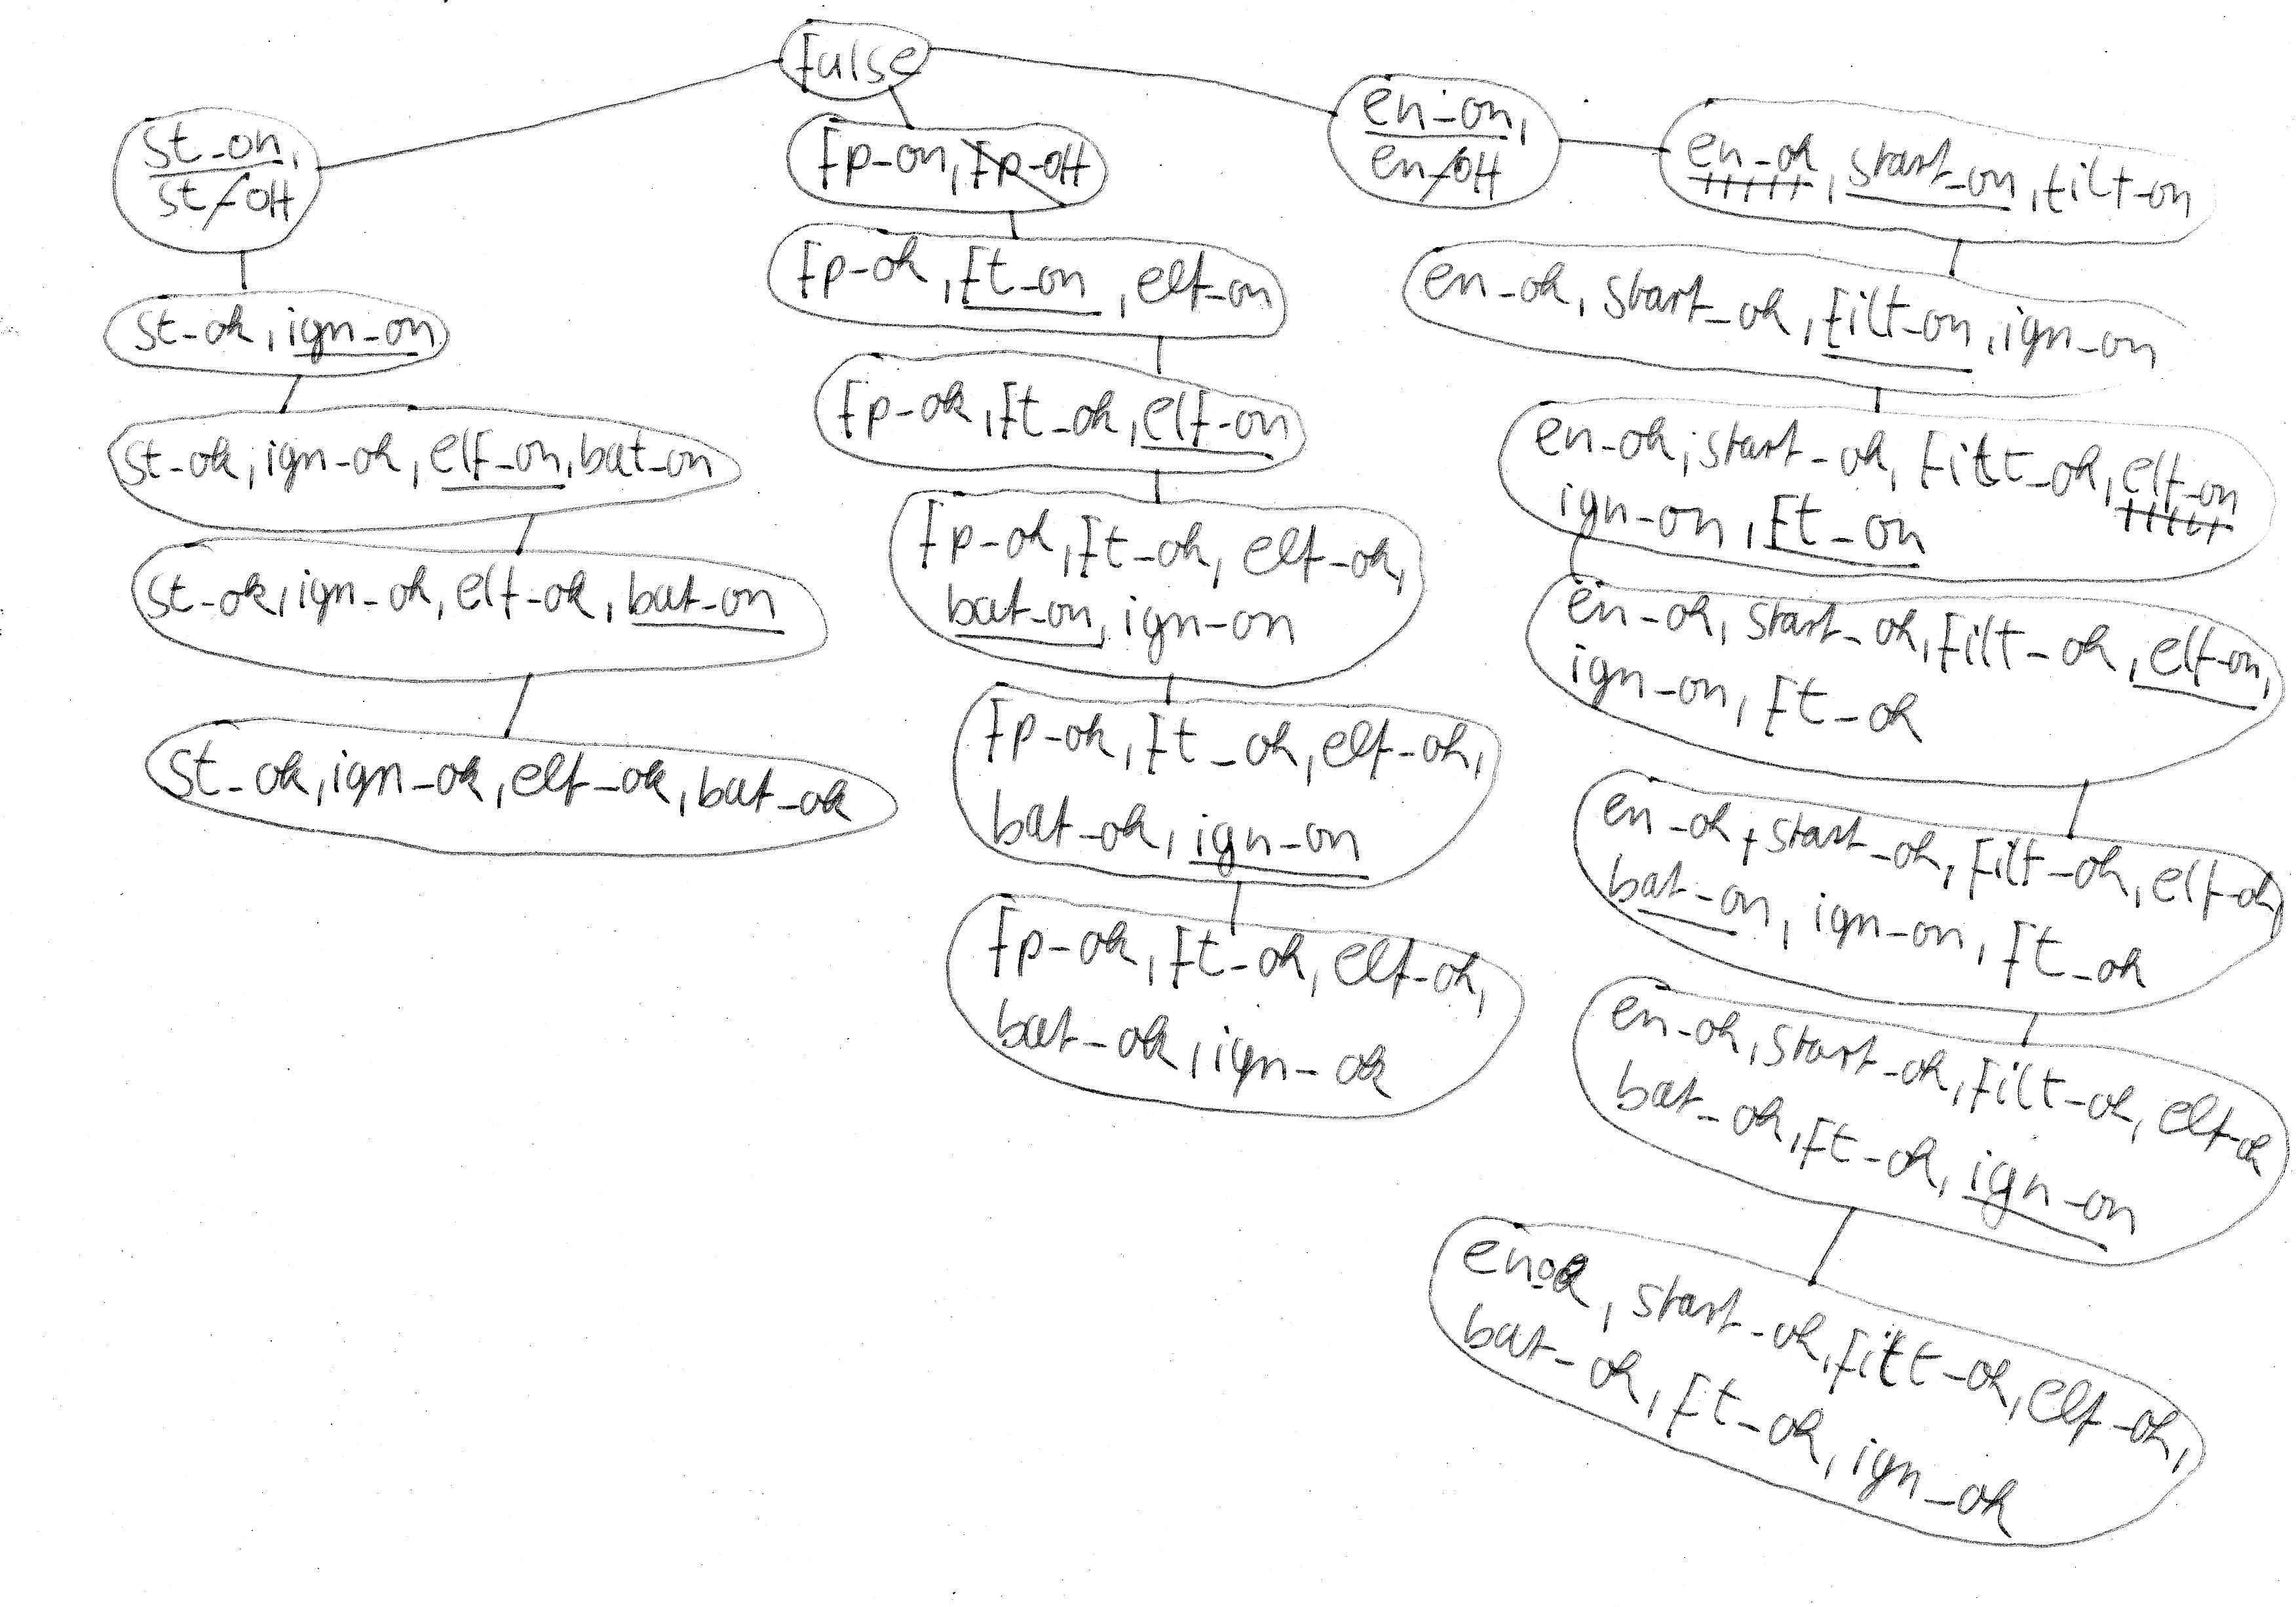
\includegraphics[width=1.5\textwidth]{baum.jpg}
%				\caption{um 30 Grad gedreht}
%				\label{fig1}
%			\end{figure}
%		
%
%		\end{landscape} 
		
		
		
		\textbf{Diagnosis}
			\begin{itemize}
				\item No noises: $starter \vee fuel \, pump \vee engine \rightarrow starter_{ok} \wedge fuel \, pump_{ok} \wedge  fuel \, tank_{ok} \wedge ignition \, key_{ok} \wedge electronic \, fuel \, regulation_{ok} \wedge  battery_{ok} \wedge filter_{ok} $ Alle Komponenten könnten kaputt sein, da die drei potenziell defekten Teile insgesamt mit allen anderen im Auto existierenden Bauteilen in direkter bzw. indirekter Verbindung stehen. Es ist nicht möglich das Problem einzugrenzen. Anders gesagt: Einer dieser Komponenten ist also nicht "`ok"' und somit wird die gesamte Struktur im Baum zu \textit{false} ausgewertet.
				
				\item Only noise 1: $starter \vee fuel \, pump \vee engine \rightarrow starter_{ok} \wedge fuel \, pump_{ok} \wedge  fuel \, tank_{ok} \wedge ignition \, key_{ok} \wedge electronic \, fuel \, regulation_{ok} \wedge  battery_{ok} \wedge filter_{ok} $ Alle Komponenten könnten kaputt sein, da die drei potenziell defekten Teile insgesamt mit allen anderen im Auto existierenden Bauteilen in direkter bzw. indirekter Verbindung stehen. Es ist nicht möglich das Problem einzugrenzen. Anders gesagt: Einer dieser Komponenten ist also nicht "`ok"' und somit wird die gesamte Struktur im Baum zu \textit{false} ausgewertet.
				
				\item Only noise 2
				
				\item Noise 1 and 2 but not noise 3
			\end{itemize}
		
		
%				battery_{on} &\leftarrow battery_{ok}\\
%				fuel \, tank_{on} &\leftarrow fuel \, tank_{ok}\\
%				starter_{on} &\leftarrow starter_{ok} \wedge ignition \, key_{ok}\\
%				ignition \, key_{on} &\leftarrow ignition \, key_{ok} \wedge electronic \, fuel \, regulation_{ok} \wedge battery_{ok} \\
%				electronic \, fuel \, regulation_{on} &\leftarrow electronic \, fuel \, regulation_{ok} \wedge battery_{ok} \wedge ignition \, key_{ok} \\
%				engine_{on} &\leftarrow engine_{ok} \wedge starter_{ok} \wedge filter_{ok}\\
%				filter_{on} &\leftarrow filter_{ok} \wedge fuel pump_{ok} \wedge fuel tank_{ok} \\
%				fuel pump_{on} &\leftarrow fuel pump_{ok} \wedge fuel \, tank_{ok} \wedge electronic \, fuel \, regulation_{ok}\\
		
		%Nennt man das so? 
	\end{enumerate}


\end{document}
